\documentclass[../fem.tex]{subfiles}

\begin{document}
\section{Postprocessing}%
\label{sec:postprocessing}

The post processing step is greatly dependent on the purpose of the FEA.
Generating graphs of the solution, or calculating errors are done in this
stage. Our implementation has a method for plotting the final solution on the
mesh, and an example of this is shown in figure \ref{fig:A_func}. Not that that
plot is not of an actual solution to this problem, but is intended to only
demonstrate the intention of this step.

\begin{Figure}
   \begin{center}
     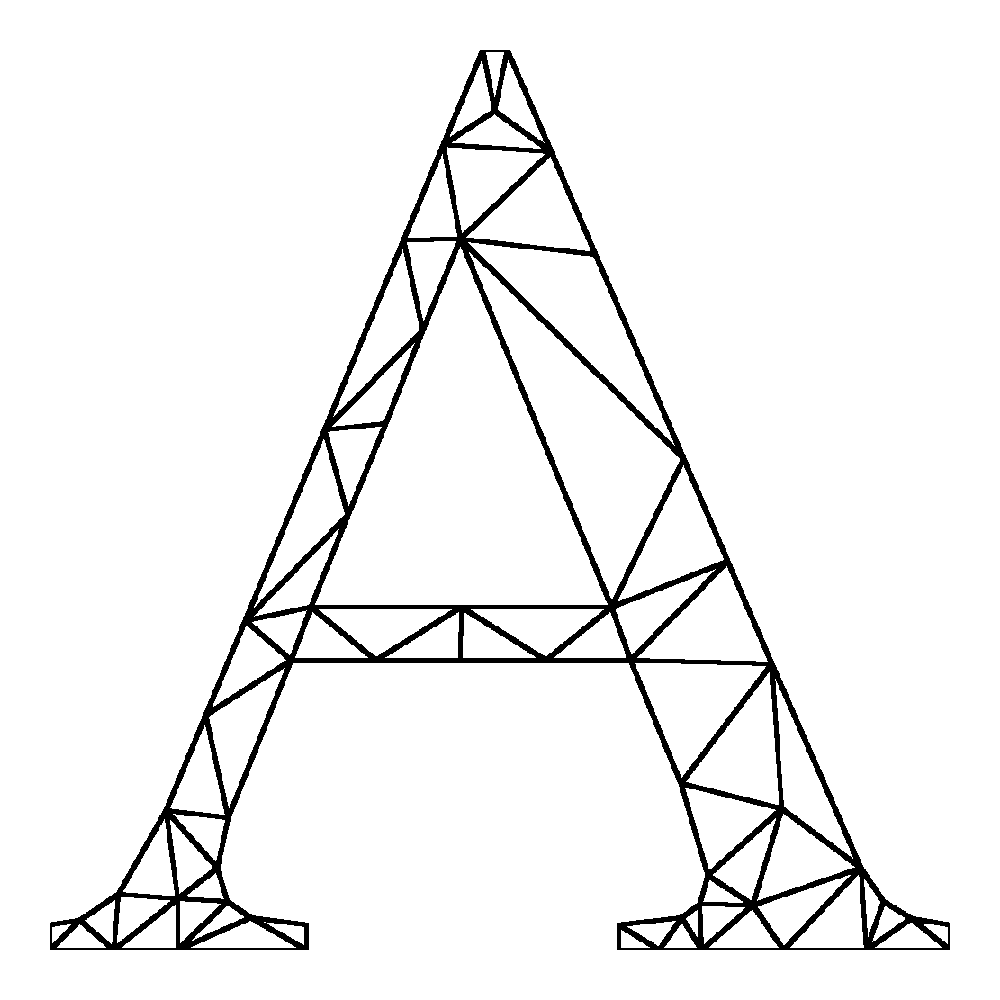
\includegraphics[width=0.8\linewidth]{a_func.png}
   \end{center}
   \captionof{figure}{Plot of the function $f(x,y)=\sqrt{x^2+y^2}$ on the mesh
   of the letter A.}\label{fig:A_func}
\end{Figure}

\end{document}
